\section{Challenge 3: 1 vs 1}

\subsection{Idea of Challenge}
% Patrick
The aim of this challenge is to have some competitive game play given the current situation.   

This challenge focuses on the following aspects:
\begin{itemize}
    \item Remote or autonomous deployment of NAO software and standardised settings for game play in a remote arena on foreign robots
    \item Automatic and semi-automatic calibration of NAO (vision, motion, etc.) 
    \item One versus One NAO competition in a ladder KO competition with all teams without much robot interaction. 
\end{itemize}

Requirements to participate in the scored part of this challenge are being able to
\begin{itemize}
    \item host an arena
    \item deploy your robot's software remotely or fully autonomous setup. 
\end{itemize}

If teams provide an autonomous setup all teams can use this to play against this in their own arena. Also teams who cannot host an arena.

\subsection{Prerequisites}
% Patrick
For this challenge teams need to fulfil multiple requirements, which are listed below in more detail.

First to be able to participate Teams have to  be able to deploy their software on the NAO remotely or you can deliver an autonomous setup. There will be several opportunities for the teams to talk, discuss, exchange ideas and code over the next few month until RoboCup. Two options will be properly available: Meetings like RoDEO and an spring RoHOW as well as to discuss on the SPL Discord channel. The second option is a code sharing section as it is available for the V6 support on RC SPL website.  

If teams are not able to participate, they (and the other teams as well) can download and deploy the images for fully autonomous setup, calibration and challenge play in the own lab. These games are not part of the ladder system and are outside of the competition.

\subparagraph*{Basic requirements for teams}

\begin{itemize}
    \item A team must be able deploy their robot software remotely or be able to produce a fully autonomous image for a robot
    \item A team must be able to host an arena. If not they have to find an substitute team, who takes over their hosting arena responsibilities.
    \item A robot must be able to semi- or fully automatic calibrate itself
\end{itemize}

\subparagraph*{Basic requirements for arenas}

The following items have to fulfilled to be able to host an arena.

\begin{itemize}
    \item A field that is nearly of the size of a 3/4 field or larger.
    \item Field marks as stated in the rules section. 
    \item Two standard goals with nets.
    \item Wifi with standard SPL\textunderscore A session, standard password and standard IP address and DHCP turned off.
    \item Remote network access via:
    \begin{itemize}
        \item VPN connection
        \item Mobile connection
        \item TeamViewer or remote desktop connection
    \end{itemize}
    \item Camera, tablet or laptop for on field online calibration with remote team using Discord.
    \item Streaming setup to stream the game on YouTube/Discord/BigBlueButton/Zoom ..., what is available (If bandwidth in the lab is limited, an restreaming should be considered on system with better network connection)
    \item Latest Game Controller running.
    \item At least 4 working NAOs V6 per game.
    \item Multiple USB Sticks with 16 GB or more memory  for flashing and logging 
    \item At least 4 balls.
    \item Assistants for remote setup and autonomous setup
    \item Referees
\end{itemize}

\subsection{Arena and organisational setup}
% Patrick
This challenge relies on a standardised arena setup as well as on exchanging all necessary information. This section provides the description for this.

\subsubsection{Data Exchange}
A NextCloud storage is used for data exchange during the days of RoboCup 2021. An access link and password will be sent to the team leaders and have to be used with care. In the NextCloud every team has its own folder (team number) which will be used for sharing the following data:

\begin{itemize}
    \item In folder \textbf{field dimensions} each team has to provide an json file (template will be given) describing the field dimensions according to the rules (TODO: link). The file has to be named \texttt{field\_dimensions.json}. This file has to be uploaded until the 15th of June 2021. The file will be used for autonomous setup and game play. To configure the arena the corresponding field dimensions json will be copied next to the image on the robot as field\_dimensions.json. This allows the usage of the same image at different arenas.
    TODO: Define Json (team name, necessary fields, wifi 2.4 or 5)
    \item  In the folder \textbf{field images} each team has a folder where photos from the arena from different angles and at different day \& night times with focus on the lighting conditions get uploaded until the 15th of June 2021.
    \item In \textbf{Robot Setup} the arena teams find an image for a particular game. Each game has an identifier and this identifier should be used as folder name. The image has to be uploaded \textbf{two hours} before the game starts.
    \item In \textbf{Arena Access} remote teams find an instruction how to access the arena. It has to contain all necessary information including usernames,  passwords or certificates. This folder in only shared with SPL teams.
    \item In the root folder you find a \texttt{streaming.md} file where every team should publish a link that can be used by public to watch the game.
    \item Logs and Images will be uploaded from the hosts into the folder \texttt{Logs/Game\_ID}, where \textit{Game\_ID} is replaced by the game identifier, after the game when bandwidth is available. It is assumed that Logs and images are stored on the USB drive attached to the NAO in the folder \texttt{logs}. Other files will be ignored.
\end{itemize}

\subsubsection{Network Setup}
The following section defines network requirements for a venue that hosts remote games. The network infrastructure should be as transparent as possible for remote participants. It should get as close as possible to an on-site experience.

\paragraph{General}

\begin{itemize}
    \item Participants need easy access to their robots for uploading code and debugging. No ports should be blocked. ICMP must not be blocked.
    \item Robots might accumulate a large amount of log files (including images). These logs are generally downloaded after games for analysis. Minimum 500Mbit/s (symmetric) is recommended for a venue, favorable 1Gbit/s.
    \item To not overwhelm the network, teams should rate limit their network activity (in particular long log downloads and uncompressed video streams from NAOs during debug sessions)
\end{itemize}

\paragraph{SPL Game specific}

\begin{itemize}
    \item Team Messages (SPLStandardMessages) must be receivable for remote participants
    \item Team Messages must not be forwarded from remote participants to 10.0.0.0/16 (SPL\_A)
    \item GameControllerMessages must be receivable for remote participants
    \item GameControllerMessages must not be forwarded from remote participants to 10.0.0.0/16 to not allow remote participants to control the game (by accident)
\end{itemize}

\paragraph{Example configuration}

\begin{figure}[ht!]
    \centering
    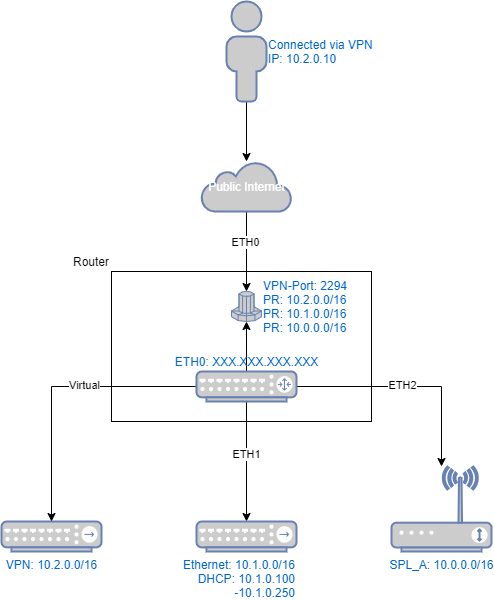
\includegraphics[width=0.5\textwidth]{figs/network.png}
    \caption{Network setup example}
\end{figure}

\begin{itemize}
    \item  The network is divided into three subnets:
    \begin{itemize}
        \item 10.0.0.0/16: The actual SPL\_A wifi network. Each team must use 10.0.TEAM\_NO.2-254 for their robots. GameController will be on 10.0.0.2. DHCP is not active.
        \item 10.1.0.0/16: The ethernet network for robots. Each team must use 10.1.TEAM\_NO.2-254 for their robots. Static addressing is required when robots are assigned to a team. DHCP is active, statically assigning 10.1.0.2-255 to robots that are currently not assigned to any team (pool).
        \item 10.2.0.0/16: The VPN network. Remote participants are assigned to this network and can access the other networks. Team- and GameControllerMessages are forwarded from 10.0.0.0/16 to this subnet. DHCP is active. Broadcasting to other subnets is not possible.
    \end{itemize}
    \item Router (e.g. Edge Router line from Ubiquity)
    \begin{itemize}
        \item serves as router for the whole network.
        \item has a globally routable (and accessible) IPv4 address.
        \item hosts an OpenVPN Layer2 VPN Server
        \item opens a network port to allow incoming OpenVPN connections
        \item Every team gets one certificate to authenticate via OpenVPN (multiple connections allowed).
        \item Has broadcast forwarding rules in place to allow VPN users to receive Team-/GC-Messages.
        \item GameController computer is assigned 10.0.0.2/16
        \item \texttt{ETH0} could be connected to your university network and is preferably accessible from the internet on the specific port (please contact your computer centre how to realise such a connection). If this is not possible, please check if you can make this network accessible from remote using a mobile internet connection. Or you provide a PC connected to an island network of this structure were people can access the PC using Teamviewer, remote desktop software, or something similar. 
    \end{itemize}
\end{itemize}

\subsection{Remote \& Game Setup}
    % - https://writemd.rz.tuhh.de/Tu3JCxovRVunD_yZwBl5Vw#
    % - https://writemd.rz.tuhh.de/rQE55j51QzqO98ifHYF0cQ#
    % - https://writemd.rz.tuhh.de/2YL-Gkz7QX2_zeJyD5Y1jA#

\subsubsection{Start: 2h before match}

    \begin{itemize}
        \item For each team two randomly selected robots are assigned from the pool
        \item Connect robot to LAN and power line
        \item Each robot gets flashed 
        \begin{itemize}
            \item with the standard Softbank image and the LAN IP address is set to 10.1.TEAM\_NO.2 and the replacement robot to 10.1.TEAM\_NO.3, if no individual image is provided by the team.
            \item with the image provided by the teams together with the field\_dimension.json and robot\_id.json indicating if the main robot or the replacement robot gets flashed. (TODO: Create json) 
        \end{itemize}
        \item Teams setup robots remotely, if necessary.
    \end{itemize}

\subsubsection{Calibration / Testing: 1 hour before match)}

    \begin{itemize}
        \item 20 min to calibrate the two robots supported by one volunteer from the hosting team. Use for communication the Discord server.
        \item  
    \end{itemize}

    Each team has 1/2 hour on full field for calibration with the help of 1 Volunteer
    Check for wifi
    Check for GC connection

Game setup

    As proposed in special corona rules
    standardized procedure for all teams (Because volunters move robots)
    Referees apply rules to prevent hardware damages (No SBR support probably)
    Longer Pause
    2 preliminary games halfes

Game end

    Teams have 10 min to clear robots (may be longer due to limited internet connection)
    Robots are returned to pool
    Next games start



\subsection{Rules}
% Arne
All rules from the current rule book apply, except for these changes:

- Starting position for robots
    - Robots start in their own half on the GC side of the field, height penalty spot

- Refereeing
    - Local team has to referee
    - Referee can prevent robot by crashing on ground if falling by catching it before
    - Team scheidet aus, wenn Laufen so schlecht, dass es zwei Spiele lange nur hingefallen ist

1. Only one field player is allowed per team. There is one replacement player.
2. The player is only allowed to stay in its own half except between the goal nets. Leaving this area results in a standard removal penalty (leaving the field).
3. The half time duration is 5 min from play (play-off-mode in GC). The game break is 5 minutes and no change of  the software is allowed. After the initial ready/set phases the game state remains in playing regardless of shot goals.
4. The game is performed with two balls on each side.
5. On each side the goal free kick positions are the starting points for the two balls.
6. Points will be counted by the referees and not by the GC.
7. Points can be scored by:
    - Shooting the ball in opponents half and it stops there (1 Point)
    - Shooting a goal (not own goal) (1 Point)
    - Touching the opponents player with the ball (0 Point)
8. If a player scores a goal (not own goal) the ball gets replaced by the referees on the starting point on its own side that is farthest from said player. The ball can directly be played again.
9. If a balls leaves the field the ball is placed on the corresponding kick in or goal free kick positions without applying the GC action (ball is instantaniously free).
10. If the score is equal for both teams the game duration gets extended for/by one minute. After each extension the score is evaluated again. At max 5 extensions are allowed. TODO: Final determination? Coin toss?
11. Teams playing with an autonomous player get a scoring factor of 2. Each point is multiplied by this factor.
12. Dive motions and wide stance is not allowed
13. Global Game Stuck

\subsection{Challenge execution}
% Arne
- Ladder system
    - KO system 
    - groups of 8 teams per Ladder
    - randomly assignement of teams to groups
    - losers of a match will play in additional ladders (To allow all teams to play at least 3 times)
    - Winners play games against each other
    - Timezones (Two games per day)
    - can only be finalized when the exact number of participants is known